% AGENTRUN -- ANTIC 2026 submission (Springer CCIS, llncs class).
% Build: pdflatex main ; bibtex main ; pdflatex main ; pdflatex main
% (or: latexmk -pdf main). See README.md.
\documentclass[runningheads]{llncs}
%
\usepackage[T1]{fontenc}
\usepackage{graphicx}
\usepackage{booktabs}
% Allow line breaks after underscores in task identifiers set in \texttt.
\usepackage[strings,nohyphen]{underscore}
\usepackage{hyperref}
\hypersetup{hidelinks}
% llncs >= 2.25 defines \Description for figure alt text (Springer
% accessibility requirement). The ANTIC-hosted llncs.cls is v2.24, which
% does not, so fall back to a no-op that keeps the alt text in the source.
\providecommand{\Description}[1]{}
%
\begin{document}
%
\title{A Trace-Level Case Study of Fine-Tuning Regression and Evaluation-Stack Confounds in a Tool-Using 7B Language Model}
\titlerunning{Fine-Tuning Regression and Evaluation-Stack Confounds}
%
\author{Alyssa L}
\authorrunning{A. L}
\institute{Department of Information Science and Engineering, Siddaganga Institute of Technology, Tumakuru, Karnataka, India\\
\email{alyssal282006@gmail.com}}
%
\maketitle
%
\begin{abstract}
Benchmark scores for tool-using language-model agents are produced by a stack of components: model weights, a tool-call parser, a client loop, tool implementations, a step budget, and a scorer. A score change between two conditions is often attributed to whichever component the experimenter intended to change. We report a small, fully traced case study that shows how fragile such attributions are. QLoRA fine-tuning of Qwen2.5-7B-Instruct on 35 tool-use trajectories lowered the pass count on a fixed 23-task multi-tool benchmark from 22 to 18. A follow-up condition (E4), intended as a parser-only ablation, re-evaluated the same adapter behind a corrected parser and also scored 18/23, while four task outcomes changed. An artifact audit then showed that E4 had been scored with a different evaluation client, with different tool schemas, message serialization and tool code, and run two weeks later against live data, so it does not isolate the parser. The recorded traces also contradict our earlier parser-based explanation of the regression. A retrained adapter (V2) with 11 failure-informed trajectories passed all 23 tasks. Exact paired tests show that none of the pairwise differences is significant at the 5\% level. We contribute the traced record, a corrected attribution, a predicate-strength audit of the benchmark, and practical checks for keeping evaluation stacks consistent before attributing a change to one intervention.

\keywords{Tool use \and LLM agents \and QLoRA \and Evaluation reliability \and Confounding \and Execution traces.}
\end{abstract}
%
\section{Introduction}
\label{sec:intro}

Language-model agents that call external tools are increasingly evaluated end to end: a task is posed, the model emits tool calls, a runtime executes them, observations are fed back, and a scorer judges the final trace~\cite{yao2023react,schick2023toolformer,mialon2023alm}. The resulting number depends on far more than the model. The tool-call parser, the client loop and its step budget, the format in which tool schemas and results are serialized into the prompt, the behaviour of the tools themselves, and the scoring predicates all sit between the weights and the score. When a score moves after an intervention, the practical temptation is to credit the component that was deliberately changed.

This paper is a case study of that temptation. It began as an engineering project that fine-tuned an open 7B model for tool use, observed a regression, attributed it partly to a brittle parser, ran a ``parser ablation'' and then a data-augmented retraining that reached a perfect score on the benchmark. A preprint of the first stage was published before the ablation was run~\cite{l2026agentrunpreprint}. A later audit of the committed artifacts, carried out before this submission, found that two key attributions were not supported. The ablation had changed the evaluation client as well as the parser, and the recorded traces of the regressed model did not show the parser failures that had been assumed. We report the full record, including what was wrong.

We address three research questions:
\begin{description}
\item[RQ1] What do the execution traces show about why the fine-tuned model regressed on this benchmark?
\item[RQ2] What can, and cannot, be concluded from the adapter-fixed comparison (E4) and from the retrained condition (V2), given how each was actually run?
\item[RQ3] How strong are the benchmark's scoring predicates, and what does that imply for interpreting pass counts?
\end{description}

Our contributions are: (i)~a fully traced record of four conditions (Base, V1, E4, V2) on a fixed, machine-checkable benchmark, with every reported number recomputed from committed artifacts; (ii)~a trace-level failure analysis that separates tool omission, step-budget exhaustion, answer wording, baseline gaps and scoring artifacts; (iii)~an audit showing that an intended single-factor ablation varied several factors, and a correction of the earlier parser-based attribution, including statements in our own preprint; and (iv)~practical checks for keeping evaluation stacks consistent. We do not claim a new method, a generalizable fine-tuning recipe, or that the parser change helps or hurts in general.

\section{Related Work}
\label{sec:related}

\paragraph{Tool use and function calling.}
ReAct interleaves reasoning traces with actions and observations, establishing the loop that most tool-using agents follow~\cite{yao2023react}. Toolformer trains a model to decide when to call APIs using self-supervised filtering~\cite{schick2023toolformer}, and Gorilla and ToolLLM fine-tune models for large API collections, evaluating with retrieval and tree-search procedures respectively~\cite{patil2024gorilla,qin2024toolllm}. API-Bank provides a benchmark with executable APIs for planning, retrieval and calling~\cite{li2023apibank}, and Mialon et al.\ survey the broader space of augmented language models~\cite{mialon2023alm}. These works establish that tool use can be learned and measured, but they mostly treat the interface between generated text and executed call as fixed infrastructure. Gorilla is an exception: it explicitly measures hallucinated API calls, a form of interface error. Our setting is far smaller. The four tools are exposed through the Model Context Protocol (MCP)~\cite{mcp2025spec}, and our question concerns how changes to that interface confound attribution, not how to improve tool use.

\paragraph{Agent benchmarks and execution-based evaluation.}
AgentBench evaluates models across eight interactive environments~\cite{liu2024agentbench}, WebArena provides self-hosted, reproducible websites so that execution-based outcomes do not drift with the live web~\cite{zhou2024webarena}, and $\tau$-bench scores tool-agent-user interactions by comparing final database state and reports a pass$^k$ reliability metric over repeated trials~\cite{yao2024taubench}. Kapoor et al.\ argue that agent evaluations focus narrowly on accuracy and ignore cost, often lack adequate holdout sets, and follow unstandardised practices that undermine reproducibility~\cite{kapoor2025agents}. WebArena's design choice to avoid live services and $\tau$-bench's repeated trials address exactly the two weaknesses our study exhibits: live tool data and a single run per condition.

\paragraph{Parameter-efficient fine-tuning and forgetting.}
LoRA trains low-rank updates to frozen weights~\cite{hu2022lora}, and QLoRA makes this feasible on a single consumer GPU by backpropagating through a 4-bit quantized base model~\cite{dettmers2023qlora}. Fine-tuning can erode prior abilities (catastrophic forgetting~\cite{kirkpatrick2017ewc}). Biderman et al.\ find that LoRA forgets less than full fine-tuning but also learns less on the target domain~\cite{biderman2024loraforgets}. Agent-specific fine-tuning such as FireAct and AgentTuning reports gains from training on agent trajectories, and AgentTuning mixes in general instruction data to retain broad ability~\cite{chen2023fireact,zeng2024agenttuning}. Our regression from Base to V1 is consistent with this literature in direction, but with a single run on 23 tasks it is not evidence for any particular mechanism.

\paragraph{Evaluation reliability and reproducibility.}
HELM argues for standardised, multi-metric evaluation and documents how prompting choices affect scores~\cite{liang2023helm}. Biderman et al.\ report that seemingly minor implementation details in evaluation harnesses change results and recommend sharing exact code and prompts~\cite{biderman2024lessons}. Sclar et al.\ show that semantically equivalent prompt formats can change few-shot accuracy substantially~\cite{sclar2024formatting}, and Tam et al.\ show that requiring structured output formats can degrade reasoning performance~\cite{tam2024speakfreely}. These findings make it plausible that changing how tool schemas and tool results are serialized, as happened in our E4 condition, could by itself change outcomes; we treat this as an alternative explanation, not a demonstrated cause. On reporting, Dodge et al.\ show that test scores alone can mislead about which model is better, and Bouthillier et al.\ show that sources of variance such as random seeds and data sampling must be accounted for when comparing models~\cite{dodge2019showyourwork,bouthillier2021variance}. Lipton and Steinhardt identify the failure to isolate the sources of empirical gains as a recurring problem in machine-learning papers~\cite{lipton2019troubling}.

\paragraph{Adaptive evaluation and leakage.}
Reusing a test set to guide model changes invalidates naive generalisation estimates~\cite{dwork2015reusable}, and benchmark leakage into training data inflates LLM scores~\cite{zhou2023cheater}. Our V2 training data were written after inspecting V1's failures on the same benchmark. That is a mild, disclosed form of adaptive analysis, and it bounds what V2's score can mean.

\paragraph{Gap addressed.}
The works above establish, separately, that infrastructure details matter and that single-run, adaptively developed results are fragile. We contribute a complete, small worked example of how these issues combined in one project. Every claim is traceable to committed artifacts, including the correction of our own earlier attribution. We see this as a cautionary case study, not a general finding.

\section{System and Methodology}
\label{sec:method}

\subsection{Task Set and Scoring}
\label{sec:tasks}

The benchmark has 23 tasks in 12 categories (Table~\ref{tab:bench}), each a single prompt answered with four tools: \texttt{calculator}, \texttt{word\_count}, \texttt{web\_search} (Tavily) and \texttt{get\_weather} (Open-Meteo). Search and weather return live data. A run is a sequence of model turns, each of which either emits tool calls or a final answer, with a budget of $m=3$ turns. For task $i$ with required tool set $R_i$, let $O_i$ be the set of tools called, $\varepsilon_i$ indicate whether any tool returned an error, $e_i$ indicate whether the task expects one, $h_i$ indicate that the budget was exhausted, and $c_i(a_i)$ be the task's content predicate on the final answer $a_i$ (substring or numeric-tolerance checks; true if none is defined). The scorer marks the task as passed iff
\begin{equation}
s_i = \mathbf{1}[R_i \subseteq O_i]\cdot \mathbf{1}[\varepsilon_i = e_i]\cdot \mathbf{1}[\neg h_i]\cdot c_i(a_i),
\label{eq:score}
\end{equation}
and a condition's result is $\sum_i s_i$ out of $N=23$, so one task corresponds to 4.35 percentage points. Unnecessary tool calls are not penalised. The predicates differ in strength (Table~\ref{tab:bench}). Fifteen tasks check answer content. Seven check only that the required tools were called, because their answers depend on live data. One no-tool task has no positive check and passes any answer that neither errors nor exhausts the budget.

The benchmark suits a case study because each outcome is decided by a small, inspectable rule and every run records the full trace. Its size and fixed composition mean that it cannot support claims about tool use in general.

\begin{table}[t]
\caption{Benchmark composition and predicate strength. ``Content'': the answer is checked by substring or numeric tolerance. ``Tools only'': only tool invocation, step budget and error status are checked. ``No check'': only error status and step budget are checked}
\label{tab:bench}
\centering
\begin{tabular}{@{}l@{\hspace{2em}}c@{\hspace{1.5em}}c@{\hspace{1.5em}}c@{\hspace{1.5em}}c@{}}
\toprule
Category & Tasks & Content & Tools only & No check \\
\midrule
math, adversarial\_math & 6 & 6 & 0 & 0 \\
text (word count) & 1 & 1 & 0 & 0 \\
weather & 2 & 0 & 2 & 0 \\
search, time\_sensitive & 3 & 1 & 2 & 0 \\
multi\_tool & 4 & 3 & 1 & 0 \\
chained\_reasoning & 1 & 0 & 1 & 0 \\
no\_tool\_expected & 2 & 1 & 0 & 1 \\
adversarial\_reasoning & 2 & 2 & 0 & 0 \\
adversarial\_error\_handling$^a$ & 1 & 1 & 0 & 0 \\
adversarial\_ambiguity & 1 & 0 & 1 & 0 \\
\midrule
Total & 23 & 15 & 7 & 1 \\
\bottomrule
\multicolumn{5}{@{}l}{\footnotesize $^a$A tool error is required for this task to pass.}
\end{tabular}
\end{table}

\subsection{Model and Fine-Tuning}
\label{sec:training}

All conditions use \texttt{Qwen/Qwen2.5-7B-Instruct}~\cite{qwen2024qwen25} loaded in 4-bit NF4 with fp16 compute. Adapters were trained with QLoRA~\cite{dettmers2023qlora} on a single Colab T4 GPU (15\,GB) using the TRL SFT trainer with a completion-only collator that masks non-assistant tokens. Both runs share the LoRA and data hyperparameters in Table~\ref{tab:train}. V1 was trained on 35 hand-written tool-use trajectories. V2 was trained on 46: the same 35 (unchanged, in order) plus 11 written after inspecting V1's failures. The 11 cover word-count-then-calculate (3), weather-then-convert (3), three-tool queries with synthesis (2), division by zero (2) and a fictional-country false premise (1). No training prompt equals a benchmark prompt after normalisation, but several share a template with a benchmark task. For example, ``What is 25 divided by 0?'' is in the training set, and the benchmark asks ``What is 50 divided by 0?''. The V2 script also enables gradient checkpointing, disables the KV cache and passes a paged 8-bit AdamW optimiser, which the V1 script does not; V1 used the trainer's default optimiser. No random seeds were set. Colab library versions were not recorded. The V2 script imports the collator from a different module path, which its comments attribute to TRL 0.14 or later. This suggests, but does not establish, that the two runs used different library versions. Both training sets regenerate byte-for-byte from the committed generator scripts.

\begin{table}[t]
\caption{Training configuration. Shared values are read from both training scripts and the saved adapter configuration}
\label{tab:train}
\centering
\begin{tabular}{@{}l@{\hspace{1.5em}}l@{\hspace{1.5em}}l@{}}
\toprule
Setting & V1 & V2 \\
\midrule
Trajectories & 35 & 46 (35 + 11 failure-informed) \\
LoRA rank / alpha / dropout & \multicolumn{2}{@{}l@{}}{16 / 16 / 0.05 (both)} \\
Target modules & \multicolumn{2}{@{}l@{}}{\texttt{q\_proj}, \texttt{k\_proj}, \texttt{v\_proj}, \texttt{o\_proj} (both)} \\
Learning rate, epochs & \multicolumn{2}{@{}l@{}}{$2\times10^{-4}$, 3 (both)} \\
Batch size & \multicolumn{2}{@{}l@{}}{2 per device $\times$ 4 accumulation = 8 (both)} \\
Max. sequence length & \multicolumn{2}{@{}l@{}}{1024 tokens (both)} \\
Optimiser & trainer default & paged 8-bit AdamW \\
Gradient checkpointing & off & on \\
Random seed & not set & not set \\
\bottomrule
\end{tabular}
\end{table}

\subsection{Serving, Parsers and Client}
\label{sec:runtime}

The model is served from Colab behind an HTTP endpoint and decodes greedily (at most 512 new tokens per turn). The server converts generated text into structured tool calls. The \emph{single-pass} parser (Base, V1) extracts only properly closed \texttt{<tool\_call>}\,\ldots\,\texttt{</tool\_call>} blocks. The \emph{two-pass} parser (E4, V2) adds a fallback that, when no closed block is found, takes the first JSON object after an opening tag. Because that fallback stops at the first closing brace, it cannot recover calls with nested arguments, so it does not recover the malformed-output case that originally motivated it. The client for Base, V1 and V2 (\texttt{ft\_agent.py}) sends the conversation and MCP-derived tool schemas to the server, executes returned calls through a local MCP server, and appends calls and observations to the conversation as \texttt{<tool\_call>} text and provider-formatted strings. Tool results beginning with \texttt{ERROR} are recorded as tool errors.

\subsection{Conditions and Evaluation Stacks}
\label{sec:conditions}

Table~\ref{tab:conditions} and Fig.~\ref{fig:stacks} summarise the four conditions. Base, V1 and V2 were run on 1~September~2026 with \texttt{ft\_agent.py} and MCP, and they record full traces. E4 was intended to change only the parser. It was scored on 16~September~2026 by an evaluation loop written inside the Colab notebook. The loop imports the task definitions and the scoring function from copies of the repository files uploaded to the session; whether those copies matched the committed versions was not recorded, although the 23 task identifiers do match. It differs from \texttt{ft\_agent.py} in four ways: its tool schemas carry one-to-three-word descriptions; it returns calls to the model as OpenAI-style \texttt{tool\_calls} and results as \texttt{\{"result": \ldots\}} JSON; it uses its own tool functions, in which only exceptions count as errors; and it has no client-side re-parse. E4 recorded pass/fail only. The same notebook also contains an E4 run made without a working search key, which scored 13/23 because search calls errored. The reported 18/23 is the run with the key working.

\begin{table}[t]
\caption{Experimental conditions. The evaluation-stack differences are summarised in Fig.~\ref{fig:stacks}}
\label{tab:conditions}
\centering
\begin{tabular}{@{}l@{\hspace{1.2em}}l@{\hspace{1.2em}}l@{\hspace{1.2em}}l@{\hspace{1.2em}}l@{}}
\toprule
 & Base & V1 & E4 & V2 \\
\midrule
Adapter & none & V1 & V1 & V2 \\
Server parser & single-pass & single-pass & two-pass & two-pass \\
Client and tools & MCP & MCP & notebook & MCP \\
Run date (2026) & 1 Sep & 1 Sep & 16 Sep & 1 Sep \\
Traces recorded & full & full & pass/fail & full \\
\bottomrule
\end{tabular}
\end{table}

\begin{figure}[t]
\centering
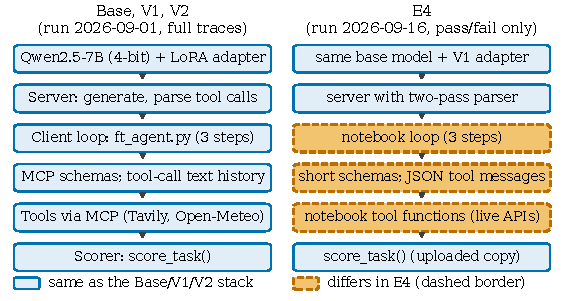
\includegraphics[width=\textwidth]{figures/fig1_eval_stacks.pdf}
\Description{Two vertical pipelines of six boxes each: model and adapter, server and parser, client loop, tool schemas and message format, tools, and scorer. In the E4 pipeline, the client loop, the schema and message format, and the tools boxes are drawn in amber with dashed borders to show that they differ from the Base, V1 and V2 pipeline; all other boxes are light blue with solid borders. A key below the pipelines explains the two box styles.}
\caption{Evaluation stacks. Amber boxes with dashed borders are components in which E4 differs from the stack used for Base, V1 and V2. The server parser also differs (single-pass for Base and V1, two-pass for E4 and V2)}
\label{fig:stacks}
\end{figure}

\subsection{Evidence and Verification}
\label{sec:evidence}

All numbers in this paper are recomputed from the committed result files~\cite{l2026agentrunrepo}. A verification script re-tallies each condition from its per-task records, checks that all four conditions contain the same 23 task identifiers, and lists every per-task transition. A CPU-only test suite pins the benchmark composition, the 35/46/11 trajectory counts, prompt-level train/benchmark disjointness and the predicate strengths in Table~\ref{tab:bench}. No experiment was re-run for this paper. In particular, the client-matched E4 described in Sect.~\ref{sec:discussion} has not been performed.

\section{Results}
\label{sec:results}

\subsection{Aggregate Outcomes}

Figure~\ref{fig:scores} and Table~\ref{tab:stats} give the pass counts. Base passed 22 tasks, V1 18, E4 18 and V2 23. Treating the 23 tasks as a sample, the 95\% Wilson intervals overlap for every pair of conditions. Exact McNemar tests on paired task outcomes give $p=0.125$ for Base versus V1 (4 tasks lost, none gained), $p=1.0$ for V1 versus E4 (2 gained, 2 lost) and $p=0.0625$ for E4 versus V2 and for V1 versus V2 (5 gained, none lost). None is significant at the 5\% level. These calculations capture only the uncertainty from sampling 23 tasks. They do not capture run-to-run variation, which is unmeasured because each condition was run once, or variation in live tool data.

\begin{figure}[t]
\centering
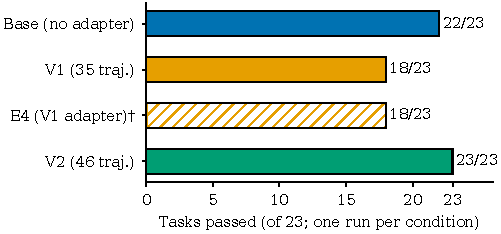
\includegraphics[width=0.62\textwidth]{figures/fig2_scores.pdf}
\Description{Horizontal bar chart of tasks passed out of 23: Base 22, V1 18, E4 18, V2 23. Bars are blue (Base), orange (V1) and green (V2); the E4 bar is white with orange hatching to mark that it used the V1 adapter under a different evaluation stack.}
\caption{Tasks passed per condition, from one run each. $^\dagger$E4 (hatched) was scored with a different evaluation client and tool stack and on a different date, so it is not directly comparable to V1}
\label{fig:scores}
\end{figure}

\begin{table}[t]
\caption{Pass counts with 95\% Wilson intervals over the 23 tasks, and exact McNemar tests on paired task outcomes (gained/lost relative to the earlier condition)}
\label{tab:stats}
\centering
\begin{tabular}{@{}lccl@{}}
\toprule
Condition & Passed & Accuracy [95\% CI] & Paired comparison \\
\midrule
Base & 22/23 & 95.7\% [79.0, 99.2] & -- \\
V1 & 18/23 & 78.3\% [58.1, 90.3] & vs.\ Base: +0/$-$4, $p=0.125$ \\
E4$^\dagger$ & 18/23 & 78.3\% [58.1, 90.3] & vs.\ V1: +2/$-$2, $p=1.0$ \\
V2 & 23/23 & 100\% [85.7, 100] & vs.\ E4: +5/$-$0, $p=0.0625$ \\
\bottomrule
\end{tabular}
\end{table}

\subsection{Task-Level Outcomes and Traces}

Only seven tasks change outcome in any condition (Fig.~\ref{fig:matrix}), and the other sixteen pass everywhere. Table~\ref{tab:traces} lists, for Base, V1 and V2, the tools called and the number of model turns for these seven tasks. E4 has no traces.

\begin{figure}[t]
\centering
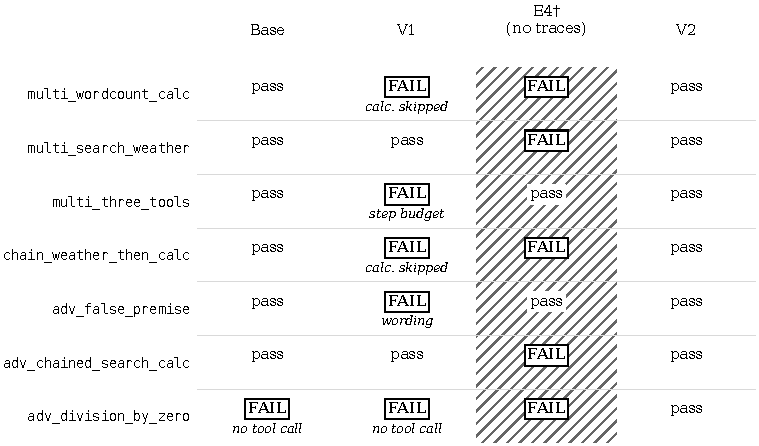
\includegraphics[width=\textwidth]{figures/fig3_task_matrix.pdf}
\Description{Grid of seven tasks by four conditions showing pass (light green box) or FAIL (bold, light red box with black border) in each cell. V1 failures are annotated with the cause seen in the trace: calculator skipped, step budget, wording, or no tool call. The E4 column is hatched and has no annotations because no traces were recorded.}
\caption{Outcomes for the seven tasks whose result differs across conditions. Italic notes give the failure cause seen in the recorded trace. $^\dagger$E4 recorded pass/fail only and used a different evaluation stack}
\label{fig:matrix}
\end{figure}

\begin{table}[t]
\caption{Trace evidence for the seven discriminating tasks: tools called, in order (turns used of 3). wc = \texttt{word\_count}, calc = \texttt{calculator}, srch = \texttt{web\_search}, wx = \texttt{get\_weather}; $\times$ = failed; ``err'' = tool returned an error}
\label{tab:traces}
\centering
\setlength{\tabcolsep}{3pt}
\begin{tabular}{@{}llll@{}}
\toprule
Task & Base & V1 & V2 \\
\midrule
multi\_wordcount\_calc & wc, calc, wc (3) & wc (2) $\times$ & wc, calc, calc (3) \\
multi\_search\_weather & srch, wx (2) & srch, wx (2) & srch, wx (2) \\
multi\_three\_tools & wx, calc, srch (2) & wx, calc, srch (3) $\times$ & wx, calc, srch (2) \\
chain\_weather\_then\_calc & wx, calc, calc (3) & wx (2) $\times$ & wx, calc (2) \\
adv.\_false\_premise & srch (2) & srch (2) $\times$ & srch (2) \\
adv.\_chained\_search\_calc & srch, calc (2) & srch, calc (2) & srch, calc (2) \\
adv.\_division\_by\_zero & -- (1) $\times$ & -- (1) $\times$ & calc err (2) \\
\bottomrule
\end{tabular}
\end{table}

\section{Failure Analysis}
\label{sec:failures}

We classify each failure by the first scoring condition in Eq.~(\ref{eq:score}) that it violates and by what the trace shows. Each category is listed with its evidence.

\paragraph{Tool omission (V1: 2 tasks).} In \texttt{multi\_wordcount\_calc} and \texttt{chain\_weather\_then\_calc}, V1 called the first tool and then did the arithmetic in prose instead of calling \texttt{calculator}, which violated $R_i\subseteq O_i$. Base and V2 called the calculator. The answers' arithmetic was not wrong in itself; the predicate requires a grounded computation.

\paragraph{Step-budget exhaustion (V1: 1 task).} In \texttt{multi\_three\_tools}, V1 used all three turns. With three calls in three turns and no final answer, it must have issued one call per turn. Base and V2 issued all three calls in a single turn and answered in the second. The failure is caused by sequential calling interacting with $m=3$. All required tools were called.

\paragraph{Answer wording (V1: 1 task).} In \texttt{adversarial\_false\_premise}, V1 searched and then answered without any accepted acknowledgement that the country is fictional.

\paragraph{Baseline gap (Base and V1: 1 task).} In \texttt{adversarial\_division\_by\_zero}, Base and V1 answered in one turn that division by zero is undefined, without calling the calculator, so the required tool error never occurred. Only V2, whose added data include two division-by-zero examples, called the tool.

\paragraph{Scoring artifacts.} Two passes are weaker than they look. In all three traced conditions, \texttt{multi\_search\_weather} passed with an answer naming a different person from the title of the top search result just received. The task has no content predicate, so the answer is never checked. V2's \texttt{adversarial\_false\_premise} answer passes because it contains the accepted substring ``Marvel'', but it never states that the country is fictional.

\paragraph{Infrastructure.} No recorded Base, V1 or V2 trace shows a tool call lost by the parser. When the server cannot parse a call, it returns the raw text as the final answer, yet none of the 69 recorded final answers contains tool-call markup. E4's four flips cannot be classified because E4 recorded no traces. The notebook's run without a working search key shows that the infrastructure alone can move the result substantially, since the same adapter and parser scored 13/23 there.

\paragraph{Correction of earlier attributions.} Our preprint~\cite{l2026agentrunpreprint}, written before E4, attributed one V1 failure to a serving-layer parsing defect on a task it called \texttt{adversarial\_search\_then\_calc}. No task of that name exists. The closest task, \texttt{adversarial\_chained\_search\_calc}, passed in the committed V1 run, with both tools called. The preprint also described V1's \texttt{multi\_wordcount\_calc} output as containing no tool-call tags, whereas the committed trace shows a \texttt{word\_count} call. The parser defect may well have been observed in a separate diagnostic run, but it is not reflected in the reported V1 results, and it should not be used to explain them.

\section{Discussion}
\label{sec:discussion}

\paragraph{What E4 does and does not show.}
With the adapter held fixed, changing the parser and the client together left the pass count unchanged while four tasks flipped. Because several components changed at once, the flips have at least four candidate explanations. The parser fallback may have extracted calls the single-pass parser missed. The shorter schemas and the JSON message format may have changed the model's behaviour, as format sensitivity results suggest is possible~\cite{sclar2024formatting,tam2024speakfreely}. Live search and weather results differed between the two dates. Greedy decoding on GPU may itself vary between runs. Every flipped task requires a tool result to be fed back to the model, which is the part of the context the notebook serialized differently, but the same is true of all 17 tool-using tasks that did not flip, so this is consistent with a client effect without being evidence for one. The experiment that would isolate the parser is the client-matched run, serving the V1 adapter behind the two-pass parser and scoring it with \texttt{ft\_agent.py} and MCP, and it has not been performed.

\paragraph{What V2 does and does not show.}
V2 passed all five tasks that failed under E4 and all five that failed under V1. Its training differed from V1 in data, optimiser and memory settings, and probably library versions, so the recovery cannot be assigned to the 11 trajectories alone. Those trajectories were written for the failure patterns observed on this benchmark, several follow the benchmark's own templates, and V2 was scored on the same 23 tasks. This is the adaptive-reuse situation that undermines holdout estimates~\cite{dwork2015reusable}. V2's 23/23 therefore shows that the identified gaps could be closed on these tasks. It does not show improved tool use in general, and with $p=0.0625$ against E4, it is not even a statistically clear improvement on this benchmark.

\paragraph{Practical checks.}
The audit suggests five checks before attributing a score change to one intervention. (1)~Run all conditions through the same client and tool code, at a recorded commit. (2)~Record full traces for every condition, not only pass/fail. (3)~Freeze or record live tool outputs, or prefer self-hosted tools~\cite{zhou2024webarena}. (4)~Report per-task transitions and paired tests alongside aggregates, and repeat runs where cost allows~\cite{yao2024taubench,bouthillier2021variance}. (5)~Audit predicate strength, so that a pass is known to mean a correct answer and not only a correct tool call. None of these is new individually~\cite{biderman2024lessons,kapoor2025agents}; the case study shows the cost of skipping them.

\section{Threats to Validity, Limitations and Ethics}
\label{sec:threats}

\emph{Internal validity.} E4 changed several factors at once. V2 changed data, optimiser and probably library versions, and its data were chosen with knowledge of the test failures. No condition was repeated, and no seeds were set. \emph{Statistical conclusion validity.} With 23 tasks and one run per condition, no difference reaches conventional significance, and run-to-run variance is unknown. \emph{Construct validity.} Eight of the 23 predicates check no answer content, and substring checks accept non-answers (Sect.~\ref{sec:failures}). The step budget of 3 penalises sequential tool calling. \emph{External validity.} The study covers one model family, one decoding mode, four tools and 23 single-prompt tasks, with no external benchmark. \emph{Reproducibility.} Code, training data, task definitions, result files, the E4 notebook (credentials redacted) and a test suite that recomputes every number are public~\cite{l2026agentrunrepo}. Training and serving need a GPU, and the live tools need network access and an API key. Re-runs should therefore be read as replication attempts, not exact reproductions. \emph{Ethics.} The study involves no human participants or personal data. The tools are benign (arithmetic, word counting, web search, weather), and no safety-critical behaviour is evaluated.

\section{Conclusion}
\label{sec:conclusion}

We traced a fine-tuning regression and its apparent repair in a tool-using 7B model and found that the most natural story, a parser bug fixed and then data added, is not supported by the evidence. The recorded failures were tool omissions, step-budget exhaustion and answer wording, not lost tool calls. The intended parser ablation changed the evaluation client too, and the perfect final score comes from a failure-informed retraining scored on the same 23 tasks, with no statistically clear gain. The main lesson is procedural: before attributing a change to one component, verify from the artifacts that the rest of the evaluation stack was the same, and inspect the traces. Justified future work is a client-matched E4 run, repeated runs per condition, recorded tool outputs, and a fresh benchmark constructed independently of the observed failures.

\begin{credits}
\subsubsection{\discintname}
The author has no competing interests to declare that are relevant to the content of this article.

\subsubsection{Use of Generative AI Tools.}
An AI coding assistant was used to audit the repository and artifacts, compute the statistics in Table~\ref{tab:stats} from committed result files, generate figure scripts, and draft and edit this manuscript. All experiments, training data and reported results predate this assistance, and the author is responsible for the content.
\end{credits}
%
\bibliographystyle{splncs04}
\bibliography{references}
%
\end{document}
